\chapter{Eksperymenty}

W niniejszym rozdziale przedstawiony został krótki opis środowiska testowego oraz przebieg testów układu do zmiany przełożeń.

\section{Środowisko testowe}
Wszystkie eksperymenty przeprowadzone zostały w sposób stacjonarny. Zamontowanie roweru na dedykowanym stojaku umożliwia swobodną symulację dowolnych scenariuszy testowych. Akwizycja danych sterownika układu jest w takim przypadku zdecydowanie mniej problematyczna, ponieważ nie jest konieczne stosowanie protokołów transmisji bezprzewodowej. 
Na potrzeby testów, autor wykonał aplikację, przedstawiającą kluczowe parametry układu w formie przebiegów czasowych. Program napisany został w języku C++, rozszerzonym o zestaw bibliotek Qt. Komunikacja pomiędzy sterownikiem a aplikacją nawiązana została za pomocą interfejsu szeregowego UART (ang. \textit{Universal Asynchronous Receiver and Transmitter}). Sterownik pracujący w trybie testowania, wysyła zastaw danych do komputera PC z częstotliwością 20Hz. Zestaw danych, składa się z chwilowych wartości:
\begin{itemize}
 \item
 kąta nachylenia podłoża,
 \item
 kadencji,
 \item
 prędkości liniowej roweru,
 \item
 wybranego biegu,
 \item
 stanu przycisku redukującego przełożenie,
 \item
 stanu przycisku zwiększającego przełożenie,
 \item
 trybu pracy sterownia.
 \end{itemize}
 
We wszystkich trybach automatycznych przedstawione są również przyjęte zakresy kadencji, a w trybie sportowym dodatkowo zakres kąta nachylenia podłoża.
 
\section{Wyniki tesów}

W niniejszym punkcie zaprezentowano wyniki testów wybranych scenariuszy, potwierdzające zgodność działania sterownika układu z założeniami, przedstawionymi w rozdziale czwartym.
\subsection{Tryb ręczny}
Podstawowa funkcjonalność układu to zmiana przełożeń w trybie ręcznym, przedstawiona na rysunku \ref{fig:tests_randomChange}:
 
\begin{figure}[h]
    \centering
    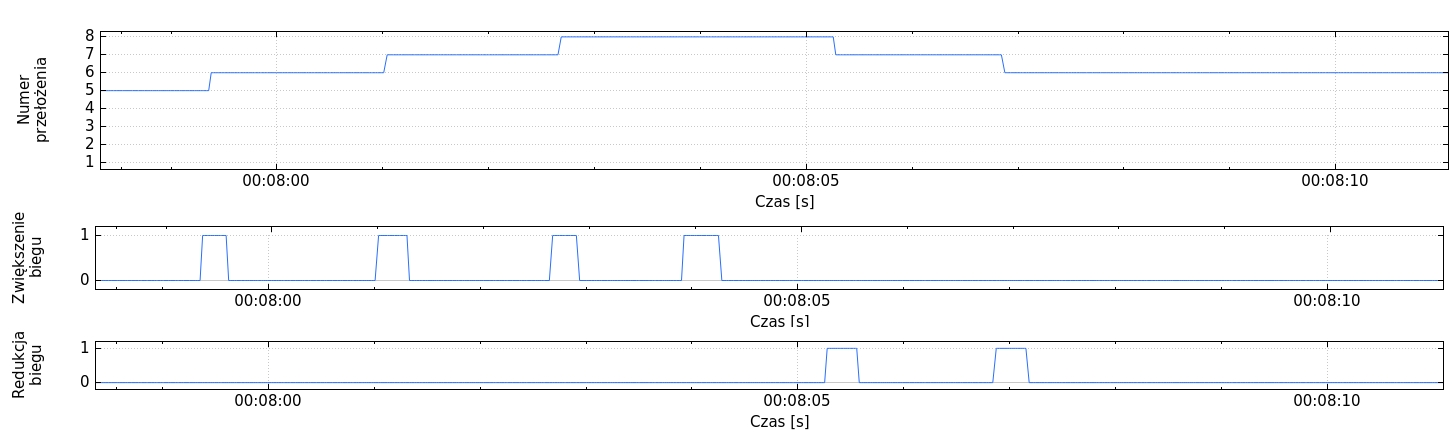
\includegraphics[scale=0.36]{tests_randomChange1.jpg}
    \caption{Zmiana przełożeń w trybie ręcznym.}
    \label{fig:tests_randomChange}
\end{figure}

Na rysunku \ref{fig:tests_continousChange} przedstawiono eksperyment potwierdzający prawidłowe działanie ciągłej zmiany przełożeń. W drugiej sekundzie testu naciśnięto i przytrzymano przycisk zwiększenia przełożenia. W efekcie co około 0.7 sekundy następuje ciągłe zwiększenie biegu od 1 do 8. Identyczne zachowanie zaobserwowano przy próbie ciągłego zmniejszenia przełożenia.

\begin{figure}[h]
    \centering
    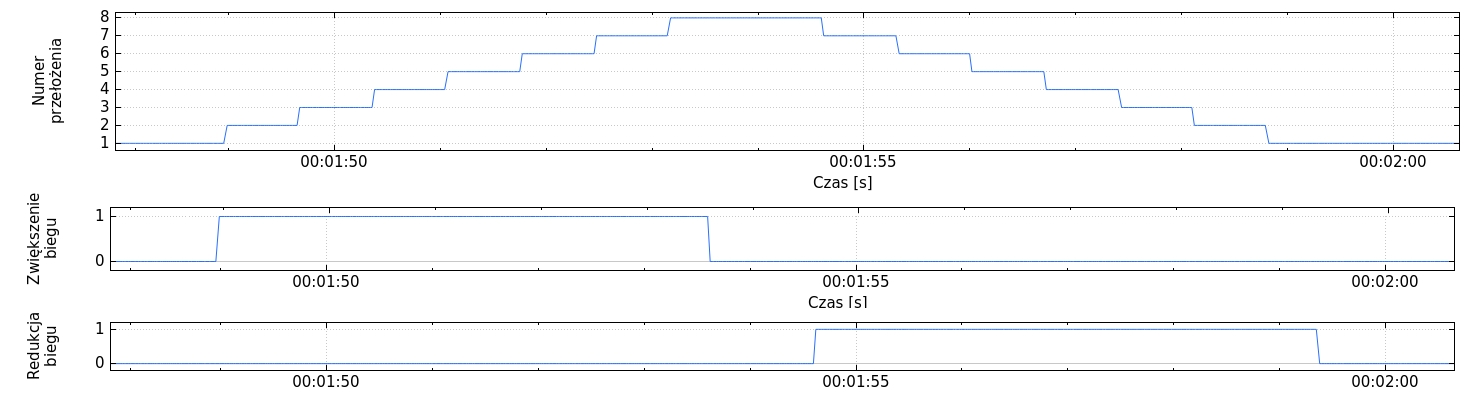
\includegraphics[scale=0.36]{tests_continousChange.jpg}
    \caption{Ciągła zmiana przełożeń w trybie ręcznym.}
    \label{fig:tests_continousChange}
\end{figure}
\subsection{Tryb comfort}

Pierwsza przetestowana funkcjonalność trybu comfort to utrzymywanie kadencji w zadanym zakresie, od $45$ do $60$ obrotów na minutę, który został oznaczony szarymi liniami. Zgodnie z przebiegami zamieszczonymi na rys. \ref{fig:tests_trybComfort}, można zaobserwować, że w wyniku przekroczenia górnej granicy wartości kadencji następuje automatyczna zmiana przełożenia. Stan przycisków do zmiany ręcznej nie zmienia się. Przełożenie zmieniane jest dwukrotnie. Kolejne zmiany przełożeń nie są konieczne w wyniku stabilizacji wartości kadencji w zadanym zakresie. 
\begin{figure}[h]
    \centering
    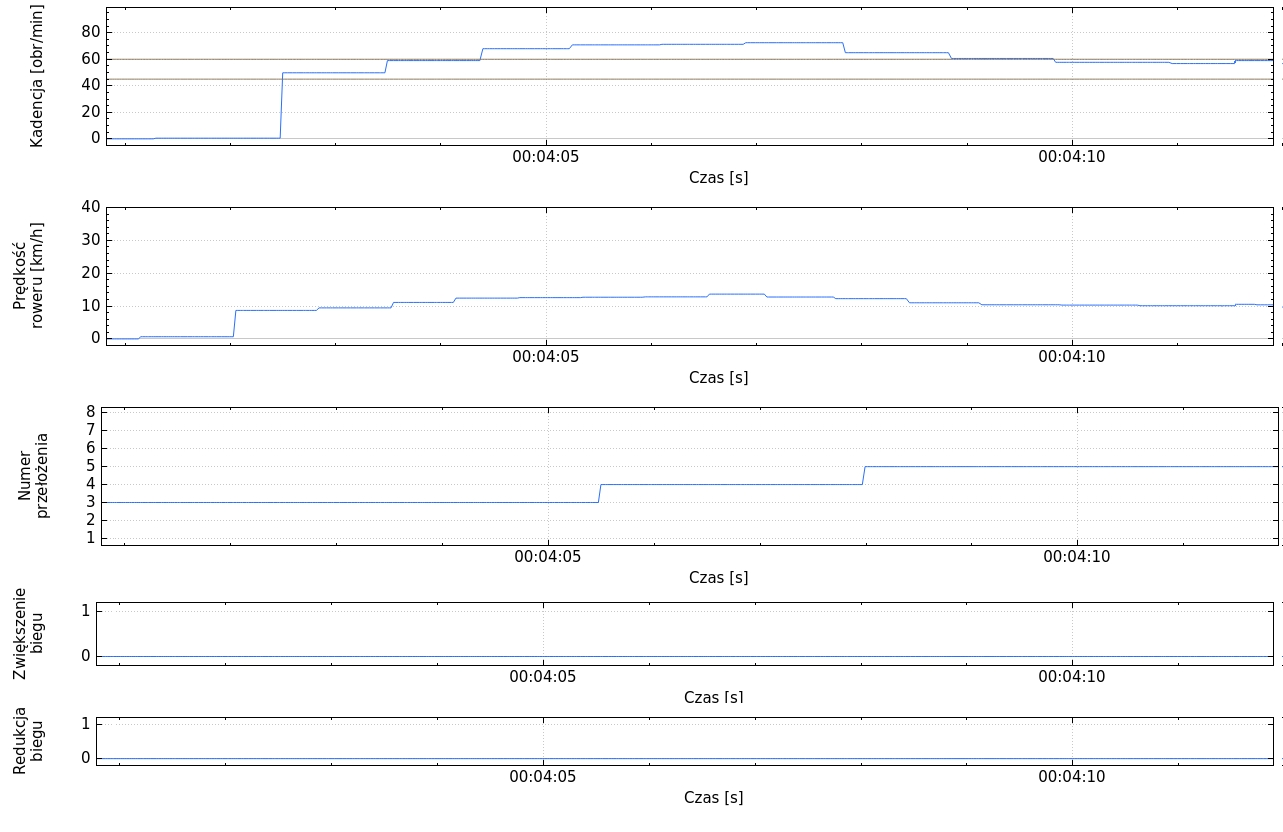
\includegraphics[scale=0.36]{tests_trybComfort.jpg}
    \caption{Automatyczna zmiana przełożeń - tryb Comfort.}
    \label{fig:tests_trybComfort}
\end{figure}

Drugi test przeprowadzony w trybie comfort obejmuje sprawdzenie wyłączenia możliwości ręcznej zmiany przełożeń, który przedstawiono na rys. \ref{fig:tests_noChange}. Przełożenie jest stałe pomimo zarejestrowanych prób ręcznej zmiany biegu.
\begin{figure}[h]
    \centering
    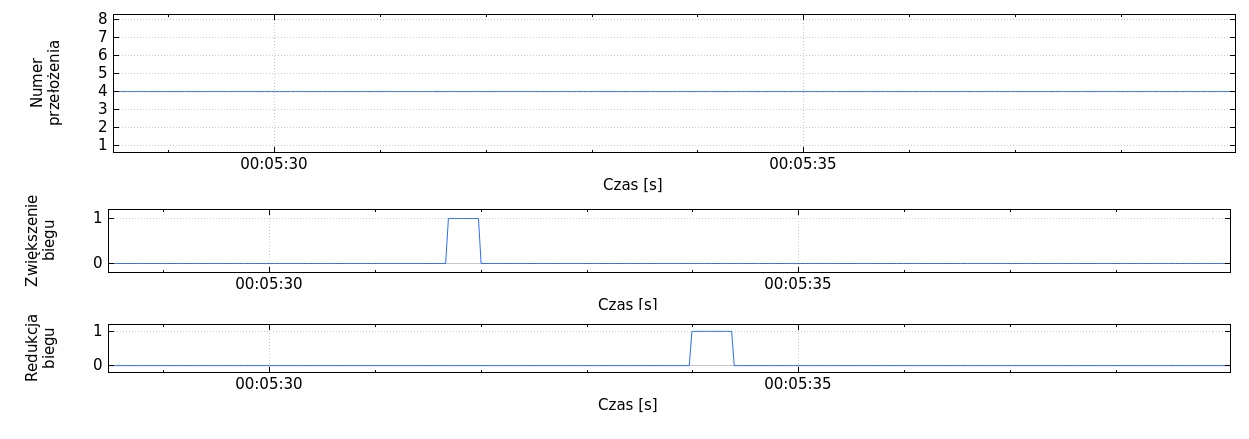
\includegraphics[scale=0.38]{tests_trybComfortBrakZmian.jpg}
    \caption{Brak reakcji na ręczną zmianę w trybie Comfort.}
    \label{fig:tests_noChange}
\end{figure}

\subsection{Tryb active}

Tryb active powinien zapewniać utrzymanie kadencji w zadanym przedziale - od 55 do 70 obrotów na minutę. Zgodnie z rysunkiem \ref{fig:tests_active}, kadencja przekracza górną granicę zakresu począwszy od czwartej sekundy testu, aż przez kolejne 10 sekund. W wyniku przekroczenia zakresu zadanej kadencji, sterownik zwiększa przełożenie do momentu, w którym kadencja ustabilizuje się w zadanym przedziale. W tym przypadku bieg nr 5 pozwala na utrzymanie kadencji w zadanym zakresie.
\begin{figure}[h]
    \centering
    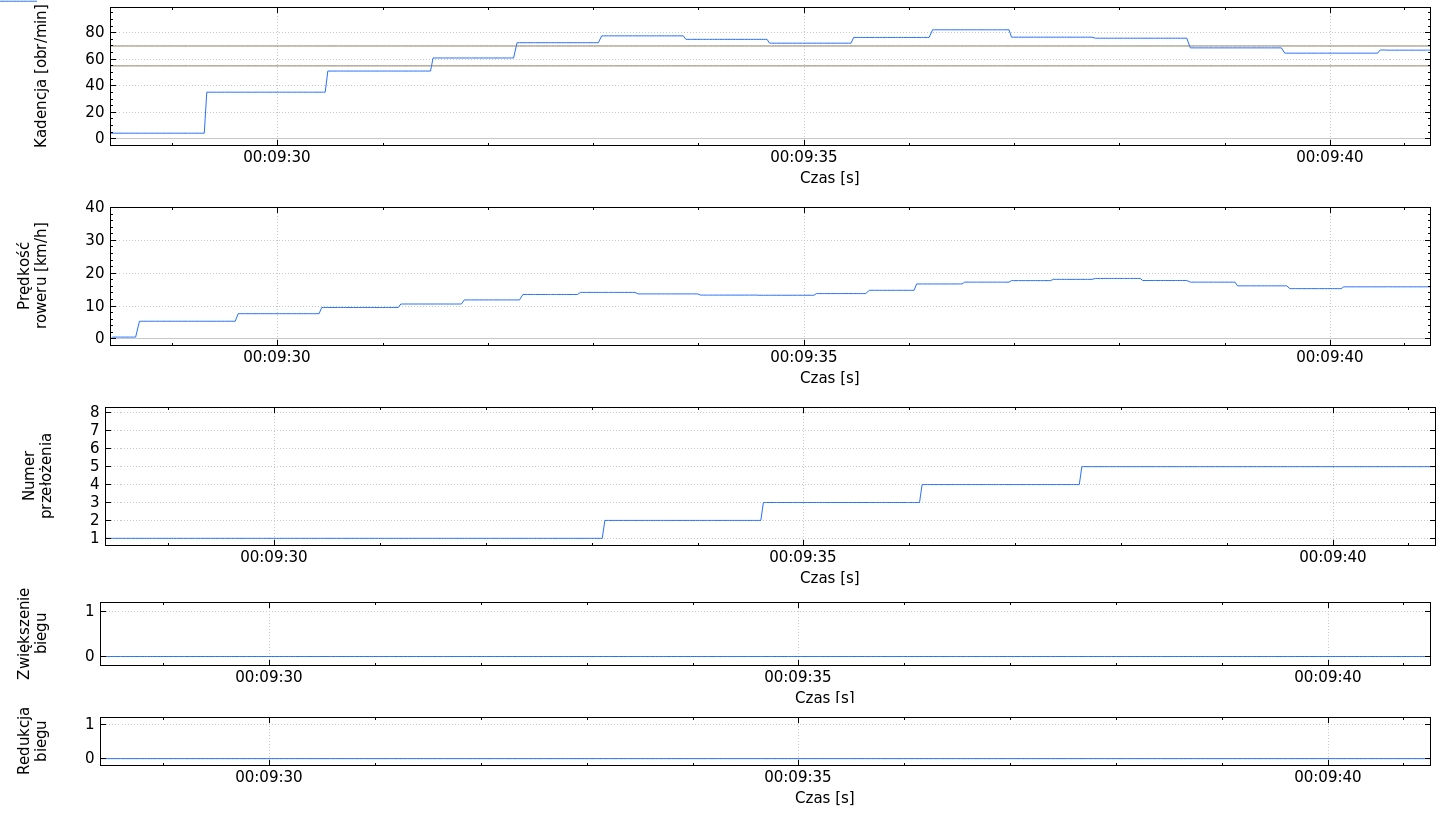
\includegraphics[scale=0.34]{tests_trybActive.jpg}
    \caption{Automatyczna zmiana przełożeń - tryb Active.}
    \label{fig:tests_active}
\end{figure}

Kolejny eksperyment miał na celu sprawdzenie możliwości ręcznej zmiany przełożeń, w wyniku której, automatyczna zmiana biegów zostaje wyłączona na 10 sekund.
\begin{figure}[h]
    \centering
    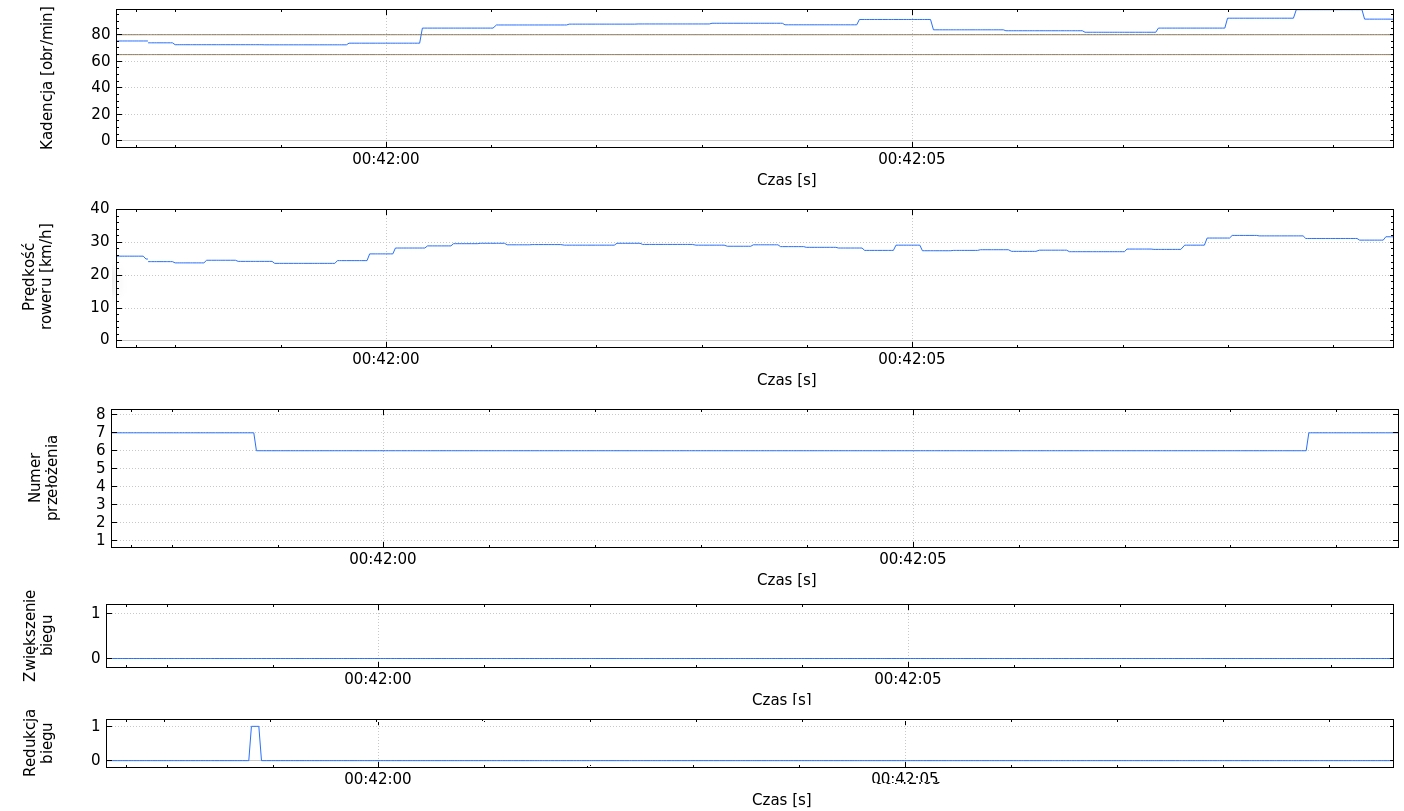
\includegraphics[scale=0.34]{tests_trybActiveRecznaZmiana.jpg}
    \caption{Ręczna zmiana przełożeń - tryb Active.}
    \label{fig:tests_activeReczna}
\end{figure}

Przebiegi, zaprezentowane na rys. \ref{fig:tests_activeReczna}, potwierdzają prawidłowe działanie sterownika. Ręczna zmiana biegu powoduje redukcję przełożenia. Pomimo przekroczenia górnej granicy zakresu kadencji, zmiana biegu następuje dopiero po 10 sekundach.


\subsection{Tryb sport}
W trybie sportowym wykonywany jest odczyt danych pomiarowych z akcelerometru i żyroskopu. Zastosowanie filtru komplementarnego, który dokonuje fuzji tych danych, umożliwia wyznaczenie kąta nachylenia podłoża (pkt.\ref{kompZasadaDzialania}). Działanie filtru można dopasować przez dobór wartości stałej czasowej. Niska wartość stałej czasowej pozwala zachować niewielkie przesunięcie fazowe pomiędzy rzeczywistą wartością kąta nachylenia a wartością estymowaną. Jednoczesnie wartość estymowana obarczona jest błędem wynikającym z dryfu żyroskopu. Wysoka wartość stałej czasowej pozwala usunąć błędy wartości estymowanej, jednak wprowadza dodatkowe opóźnienie. Dobór tego parametru jest zależny od aplikacji.

Kąt nachylenia podłoża, po którym porusza się rower, jest wielkością wolnozmienną, w porównaniu do np. kątów określających orientację wielowirnikowych platform latających. Niwelowanie błędu wynikającego z dryfu oraz przyspieszeń dynamicznych, działających na akcelerometr jest ważniejsze, niż szybka odpowiedź filtru. Dlatego stała czasowa powinna przyjąć wysoką wartość. Przebiegi przedstawione na rys. \ref{fig:tests_imu1} oraz \ref{fig:tests_imu2} przedstawiają przebieg estymowanej wartości kąta nachylenia podłoża dla przypadków, w których stała czasowa wynosi odpowiednio $0.5$ i $2$ sekundy, a wartość kąta nachylenia nie ulega zmianie:
\begin{figure}[h]
    \centering
    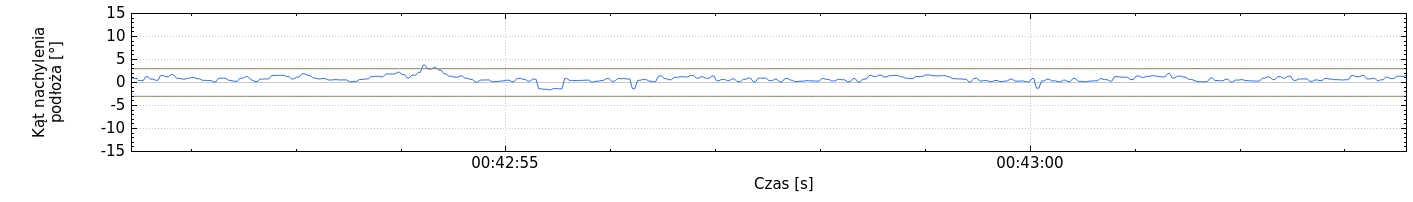
\includegraphics[scale=0.34]{tests_imu1.jpg}
    \caption{Przebieg estymowanej wartości niezmieniającego się kąta nachylenia dla stałej czasowej równej 0.5 sekundy.}
    \label{fig:tests_imu1}
\end{figure}

\begin{figure}[h]
    \centering
    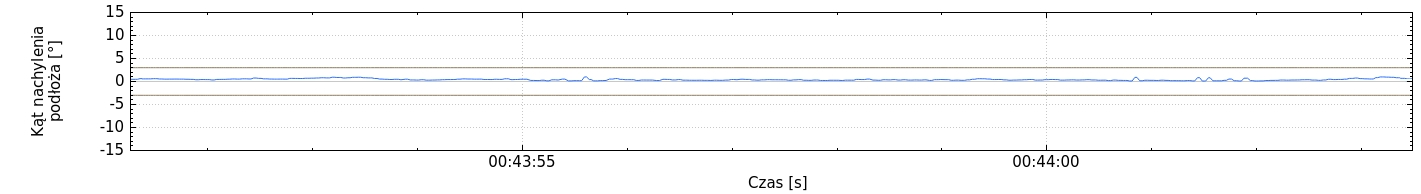
\includegraphics[scale=0.34]{tests_imu2.jpg}
    \caption{Przebieg estymowanej wartości niezmieniającego się kąta nachylenia dla stałej czasowej równej 2 sekundy.}
    \label{fig:tests_imu2}
\end{figure}
Stała czasowa ustalona na poziomie $0.5$ sekundy jest zdecydowanie za mała. Zaobserwowano znaczące błędy estymacji, spowodowane  przyspieszeniami działającymi na jednostkę pomiarową, które są efektem niewielkich ruchów roweru w trakcie przeprowadzania eksperymentu. Estymowana wartość kąta nachylenia przekroczyła, w drugiej sekundzie testu, granicę trzech stopni. Taki sposób działania filtru komplementarnego w skuteczny sposób zakłóca pracę sterownika, ponieważ zakres oczekiwanej kadencji zmienia się pomimo braku zmian wartości kąta nachylenia. Zwiększenie stałej czasowej do 2 sekund powoduje znaczącą poprawę działania filtru. Obserwowane są minimalne odchylenia estymowanej wartości kąta nachylenia. Można przeprowadzić bardziej wyczerpującą analizę problemu doboru stałej czasowej, która prowadzi do wyznaczenia wartości optymalnej, z punktu widzenia przyjętych wskaźników jakości. Jednak wymaga ona precyzyjnego mechanizmu umożliwiającego pomiar rzeczywistych wartości kątów określających orientację układu pomiarowego. Autor uznał, że osiągnięta precyzja jest w pełni wystarczająca do poprawnego działania kontrolera.



W trybie sport zakres zadanej kadencji jest zależny od wartości kąta nachylenia podłoża - tj. od 65 do 80 obrotów na minutę, jeśli wartość bezwzględna kąta nachylanie jest mniejsza bądź równa 3$^{\circ}$, oraz od 55 do 70 obrotów na minutę w pozostałych przypadkach. Przebiegi przedstawione na rys.  \ref{fig:tests_sportModeZmiana1} i \ref{fig:tests_sportModeZmiana2} potwierdzają poprawne działanie kontrolera.
\begin{figure}[h]
    \centering
    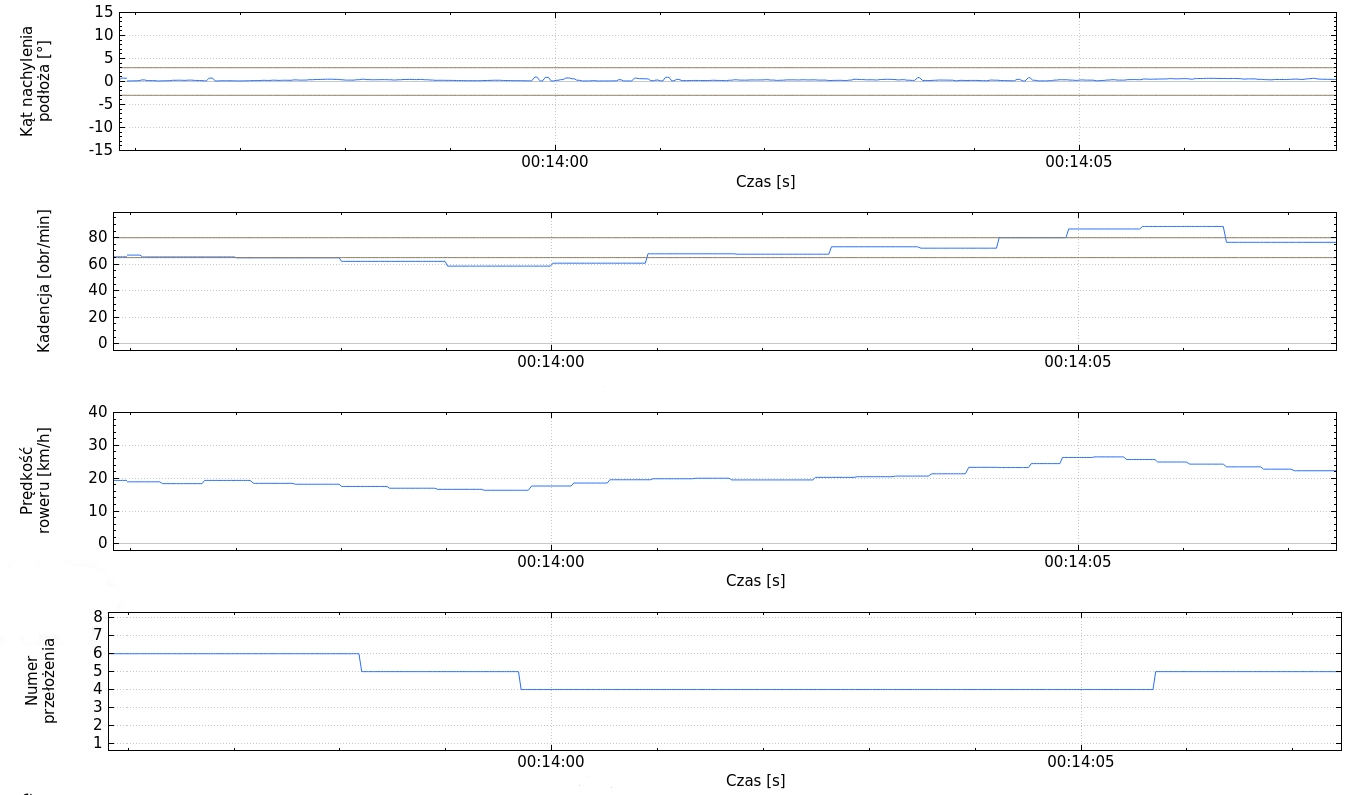
\includegraphics[scale=0.34]{tests_trybSportZmianaBiegow.jpg}
    \caption{Automatyczna zmiana przełożeń - tryb Sport}
    \label{fig:tests_sportModeZmiana1}
\end{figure}
Pierwszy przebieg zarejestrowano dla stałej wartości kąta nachylenia. Można zauważyć, że przełożenie zmieniane jest, gdy aktualna wartość kadencji jest poza zakresem 65-80 obrotów na minutę. 
\begin{figure}[h]
    \centering
    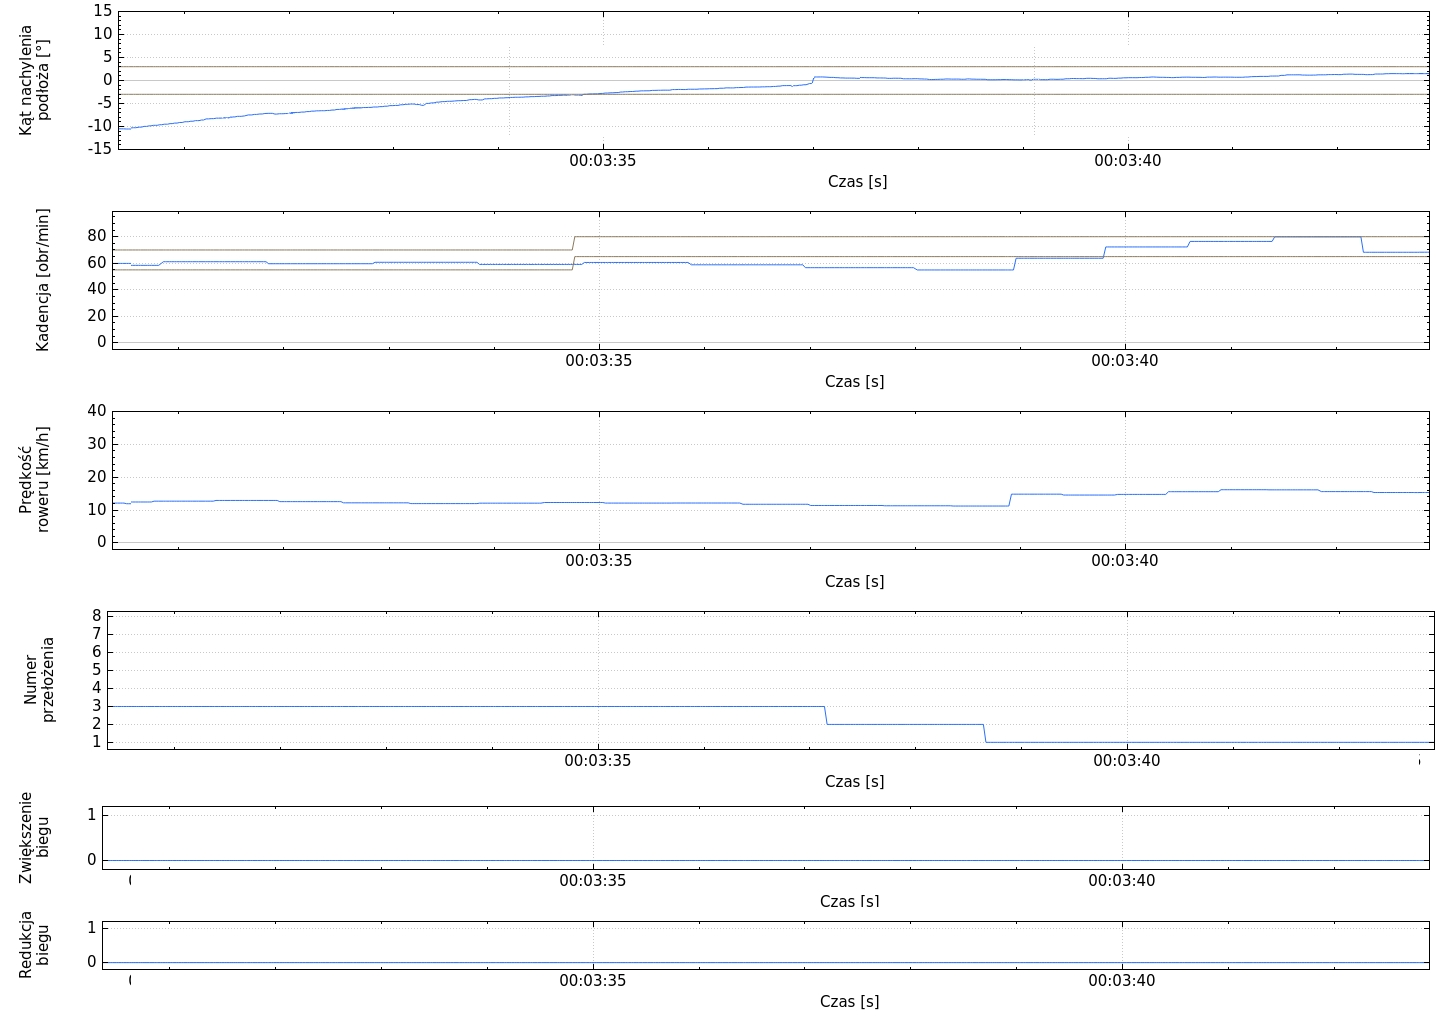
\includegraphics[scale=0.34]{tests_trybSportKat.jpg}
    \caption{Zmiana zakresu zadanej kadencji wraz ze zmieniającą się wartością kąta nachylenia podłoża.}
    \label{fig:tests_sportModeZmiana2}
\end{figure}

Drugi przebieg przedstawia symulację zjazdu roweru ze zbocza o znacznym nachyleniu. Jednostka pomiarowa IMU została zamontowana w taki sposób, aby umożliwić jej obrót wokół osi $Z$. Dzięki temu możliwa jest symulacja zmiany kąta nachylenia podłoża w przypadku, gdy rower zamontowany jest na stanowisku testowym. Także w tym przypadku kontroler działa zgodnie z założeniami. Początkowo wartość kąta nachylenia wynosi około -10$^{\circ}$. Kadencja utrzymana jest w niższym zakresie obrotów. Kąt nachylenia zaczyna rosnąć. W momencie, w którym jego wartość jest większa niż -3$^{\circ}$, następuje zmiana zakresu zadanej kadencji, której aktualna wartość jest niższa od oczekiwanej. W wyniku uruchomienia zadania cyklicznego dla trybu sport następuje redukcja przełożenia.

Ostatnia z testowanych funkcjonalności to dobór przełożenia, zależny od prędkości roweru, po wznowieniu pedałowania. Ta funkcjonalność działa w takim sam sposób w trybie active oraz sport.
\begin{figure}[h]
    \centering
    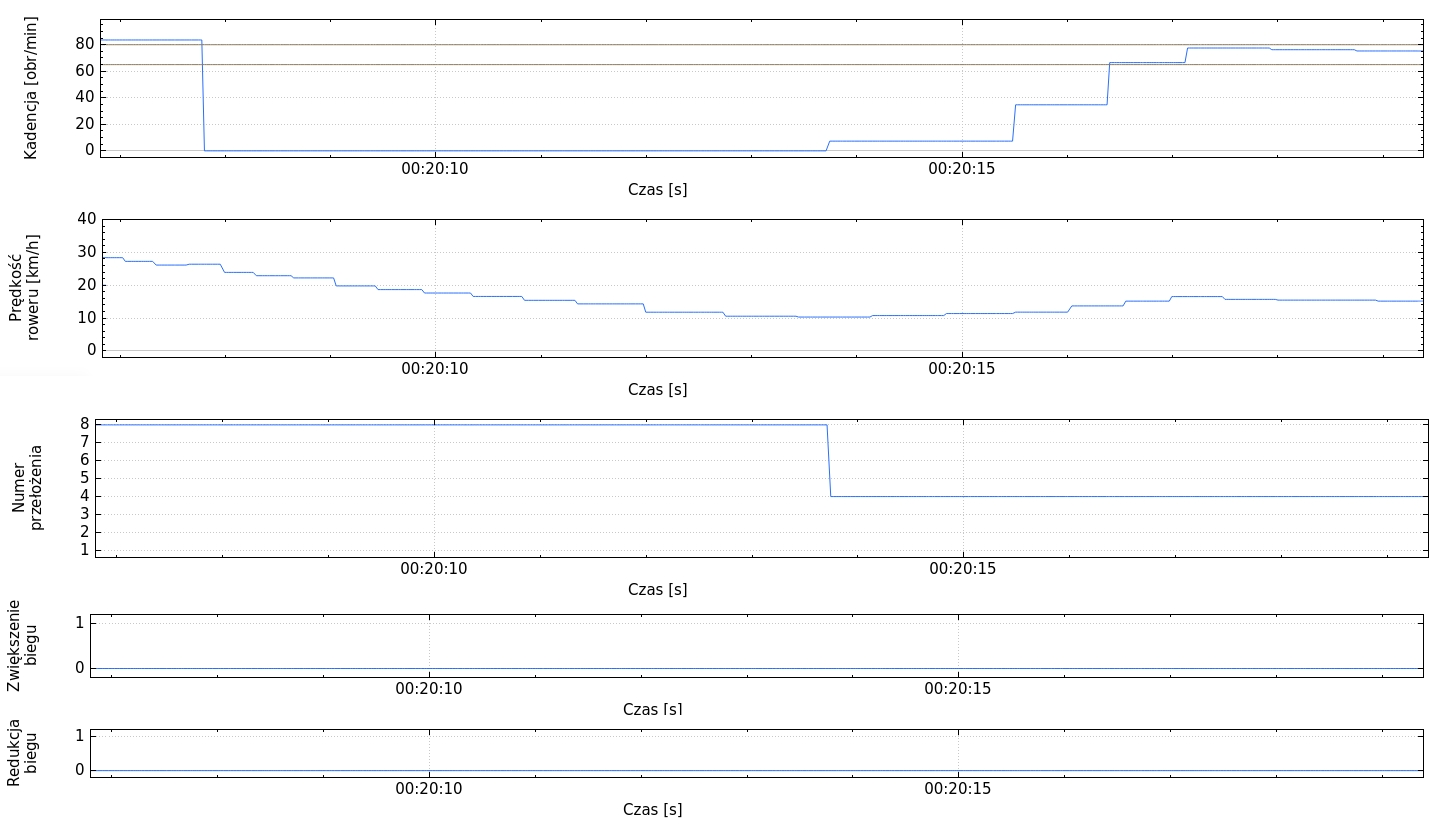
\includegraphics[scale=0.35]{tests_trybSportDopasowanieBiegu.jpg}
    \caption{Dopasowanie przełożenia w wyniku zatrzymania pedałowania - tryb Sport.}
    \label{fig:tests_gearSpeedSelection}
\end{figure}

Przebiegi, zamieszczone na rys. \ref{fig:tests_gearSpeedSelection}, przedstawiają działanie kontrolera w sytuacji, gdy następuje wznowienie pedałowania po przerwie trwającej dłużej niż 2 sekundy. W wyniku tej przerwy wartość kadencji jest ustawiana na 0. Biegi nie są zmieniane aż do pierwszego zwarcia czujnika magnetycznego. Oznacza to wznowienie pedałowania, a co za tym idzie możliwość zmiany przełożeń. Prędkość roweru w tym momencie wynosi 10$\frac{km}{h}$. Zgodnie z tabelą \ref{tab:zakresOdPredkosci}, kontroler ustawia bieg nr 4. W trakcie prac nad tą funkcjonalnością okazało się, że po wznowieniu pedałowania może dochodzić do dwóch zmian przełożenia w niewielkim odstępie czasu. Przyczyną tego problemu jest dopasowanie przełożenia do prędkości, które może nastąpić w dowolnym momencie, oraz cykliczne zadanie trybu sport. Aby tego uniknąć, pierwsze działanie zadania cyklicznego po wznowieniu pedałowania jest pomijane. Takie zachowanie jest widoczne na rys. \ref{fig:tests_gearSpeedSelection}. Zadanie cykliczne uruchamiane jest co 2.5 sekundy. Po wznowieniu pedałowania kadencja utrzymywana jest poniżej zadanej wartości przez dłuższy czas - około 3 sekundy. Zatem w tym czasie na pewno uruchomione zostało zadanie cykliczne. W celu wyeliminowania zmian przełożeń częstszych, niż 2.5 sekundy, pierwszy cykl został pominięty i nie doszło, w tym przypadku, do redukcji przełożenia.







